\Chapter{Ütközésvizsgálat}
\label{Chap:utkozesvizsgalat}

Ebben a fejezetben az ütközésvizsgálattal kapcsolatos számításokról, optimalizációkról lesz szó. Ütközésvizsgálatra több szempontból is szükség van. Egyrészt, vizsgálni kell, hogy a játékos a játszható területen belül van-e, azaz nem mehet át falakon, tereptárgyakon, nem mehet fel túl meredek emelkedőn. Másrészt, vizsgálni kell, hogy a játékos által leadott lövedék eltalálja-e a domborzatot, tereptárgyakat, jelezni kell a lövedék becsapódását. Harmadrészt regisztrálni kell az ellenfeleket eltaláló leadott lövéseket. A második és harmadik pont nagyon hasonló, de mégis célszerűnek tűnt külön kezelni. A magasságmező és az egyéb modellek ütközésvizsgálatának módját azért érdemes külön kezelni, mert a statikus magasságmező esetében másfajta optimalizálási módok állna rendelkezésre, mint az egyéb tereptárgyak, és animált karakterek esetében.

\section{A karakterek ütközésvizsgálata mozgás szempontjából}

Ez a játék szempontjából az egyik legfontosabb elem, mivel ez adja a virtuális világ egyfajta realitását. Az, hogy kirajzoltatunk valamit a képernyőre, még nem jelenti azt, hogy azon nem lehet áthaladni. Konkrétan a Z-buffer felelős azért, hogy a takarási feladatot megoldja, viszont azt úgy képes végrehajtani, hogy közben a kirajzolt objektumok ütközését a lehető legegyszerűbb módon kezeli csak.

A kirajzolás csak a vizualitást adja, a domborzat, a tereptárgyak, a karakterek kinézetét. A játékfejlesztő feladata az, hogy megírja külön az ezekhez szükséges ütközésvizsgálatot. Mivel ez két különálló dolog, egyes helyzetekben adódhatnak olyan problémák, hogy ezek nincsenek szinkronban, tehát látunk valamit amin át lehet menni, vagy nem látunk valamit és mégis megakadunk benne.

A szakdolgozat készítése közben fejlesztett játékmotorban a karakterek és a magasságmező ütközését magasságpontok és az ezek különbségeiből kapott gradiensek számításával oldottam meg. Ez azt jelenti, hogy ha két, egymás mellett lévő pont magasságértéke között túl nagy a különbség pozitív irányba, az falat, vagy túl meredek emelkedőt jelent. Ez a különbség tehát az eredeti felület pontbeli gradiensének numerikus közelítését adja. Ha mérsékelt, vagy nagyon minimális a különbség, akkor arról vagy lecsúszik, vagy csak egyszerűen át lehet ott haladni. Mindezt a beolvasott magasságmezőből számolja, így az ütközésvizsgálat minden új magasságmező esetében automatikusan elérhető.

Jelölje $H$ azt a két változós valós függvényt, amelyet a magasságmezővel közelítünk. Legyen a $\widetilde{H}$ az az interpolációs függvény, amelyeket az interpoláció alappontjaiban felveszik a $H$ értékét. Egy $p \in \mathbb{R}^2$ pozíció esetén a pontbeli gradienst a következő módon közelíthetjük:
$$
\nabla H(p) =
\left( \dfrac{\partial H(p)}{\partial x}, \dfrac{\partial H(p)}{\partial y} \right)
\approx
\left(
\dfrac{\widetilde{H}(p + \delta_x) - \widetilde{H}(p)}{\delta_x},
\dfrac{\widetilde{H}(p + \delta_y) - \widetilde{H}(p)}{\delta_y}
\right),
$$
ahol $\delta_x$ és $\delta_y$ az $x$ és $y$ tengely szerinti tetszőlegesen kis eltolást jelöli.

A gradiens közelítésének ez az egyik legegyszerűbb módja. Előnyös, mivel az interpolált felület pontbeli értékeit egyébként ki kell számítani, illetve a számítási pontosság megfelelő a játékmotor működéséhez.

Ezen felül a gravitáció ami nagyon lényeges, mert a pályának vannak olyan magaslati pontjai, amelyekre fel lehet jutni. Ha egy ilyenre felmegyünk, és nincs semmilyen erő, ami a karaktert a föld felé húzná, akkor felfelé ugyan lekövetné a talajmagasságot, de le már nem tudna esni.

A játékmotor fizikájában egy lefelé ható erő folyamatosan hat a játékosra és ellenfelekre, aminek a küszöbértéke mindig az aktuális talajmagasság. Ugrás esetén a gravitációnál nagyobb, ellenirányú erőt fejt ki a karakter, amely folyamatosan csökken. Ez eredményezi azt, hogy elemelkedik a földtől, egy ponton megáll, majd vissza is esik a talajra. Ez látható \aref{fig:gravity}-es ábrán. A gravitációs erőt az $F_g$ jelöli, a kifejtett erőt pedig az $F_k$.

\begin{figure}[h]
\centering
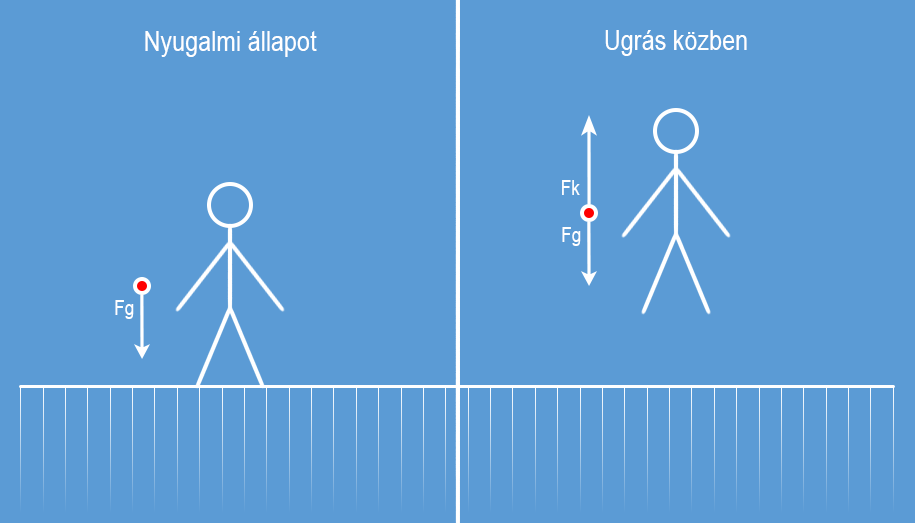
\includegraphics[scale=0.6]{kepek/gravity.png}
\caption{A karakterre ható erők}
\label{fig:gravity}
\end{figure}

A karakter függőleges pozícióját jelöljük $z$-vel. Amennyiben a játékos a magasságmezőn áll, akkor teljesül, hogy $\widetilde{H}(p) = z$. Az $F_g$ gravitációs erőt konstansnak tekintjük. Ennek tipikusan csak $z$ tengely irányú, $0$-tól különböző komponense van. Amennyiben a karakter a magasságmező felett van, úgy a $z$ és az $F_k$ is felírható az idő függvényében $t$ szerint. Egy $\Delta t$ mintavételezési időt feltételezve (ami tipikusan a képkockák kirajzolásai között eltelt idő) a következő összefüggéseket írhatjuk fel:
\begin{align*}
F_k(t + \Delta t) &= F_k(t) + F_g \cdot \Delta t, \\
z(t + \Delta t) &= z(t) + F_k(t) \cdot \Delta t. \\
\end{align*}
Amikor tehát a karakter a magasságmezőre érkezik, akkor az $F_k$ értékét $0$-nak tekinthetjük, a $z$-t pedig a magasságmező adott pontjának értékére állíthatjuk.

A koordinátarendszer és az erők mértékegységének megfelelően szükségünk lehet korrekciós szorzókra, például ha méterben és másodpercben szeretnénk számolni.
 
\section{A domborzat és tereptárgyak üközésvizsgálata a lövés szempontjából}

A domborzattal való ütközésvizsgálat azért fontos, hogy azon keresztül ne lehessen eltalálni az ellenfeleket, illetve ezzel is realisztikusabbá tehetjük a játékot. A nagy poligonszám miatt ez is optimalizációt igényel.

A problémát az egyenes és a háromszög metszéspontjának számítására vezethetjük vissza. A domborzat háromszögeit fekete szegélyekkel láthatjuk \aref{fig:wireframe} ábrán.

\begin{figure}[h]
\centering
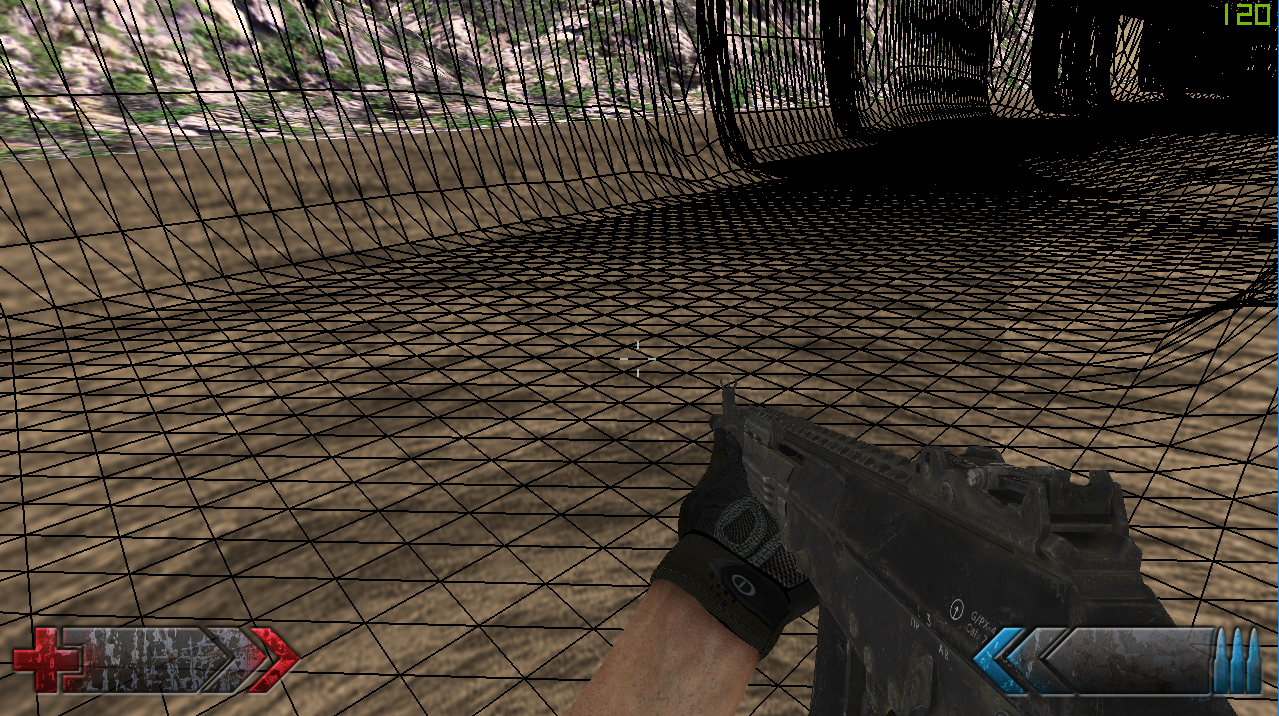
\includegraphics[scale=0.4]{kepek/map_wireframe.png}
\caption{A térkép geometriájának határvonalai}
\label{fig:wireframe}
\end{figure}

\subsection{Program: Ütközésvizsgálat}

Első lépésként, meg kell határozni azt az egyenest, amely azt írja le, amerre néz az adott karakter. Az egyenes megadható két pontjával. Az egyik az adott karakter pozíciójával egyezik meg. A másik, távoli pontot jelen esetben egy, az OpenGL-ben definiált függvényből, a \texttt{GluLookAt} függvényből határozzuk meg, aminek 9 paramétere van. Az első három a karakter jelenlegi pozíciója, a második három azt a pontot írja le merre nézünk (referencia pont), az utolsó három pedig azt határozza meg, hogy melyik tengelyen, és merre néz a felfelé vektor. A 9 paraméter közül a középső háromból lehet a második pontot  meghatározni.

Második lépésként ki kell számolni ennek az egyenesnek a háromszögekkel vett metszéspontját. A háromszögeket a három csúcspontjukkal írjuk le. Kell lennie egy függvénynek, amelynek a háromszög három csúcspontját, és az egyenes két végpontját átadva, visszakapjuk a metszéspont $(x, y, z)$ koordinátáját. A számítás eredményének egy szemléltetését \aref{fig:triangle} ábrán láthatjuk.

\begin{figure}[h]
\centering
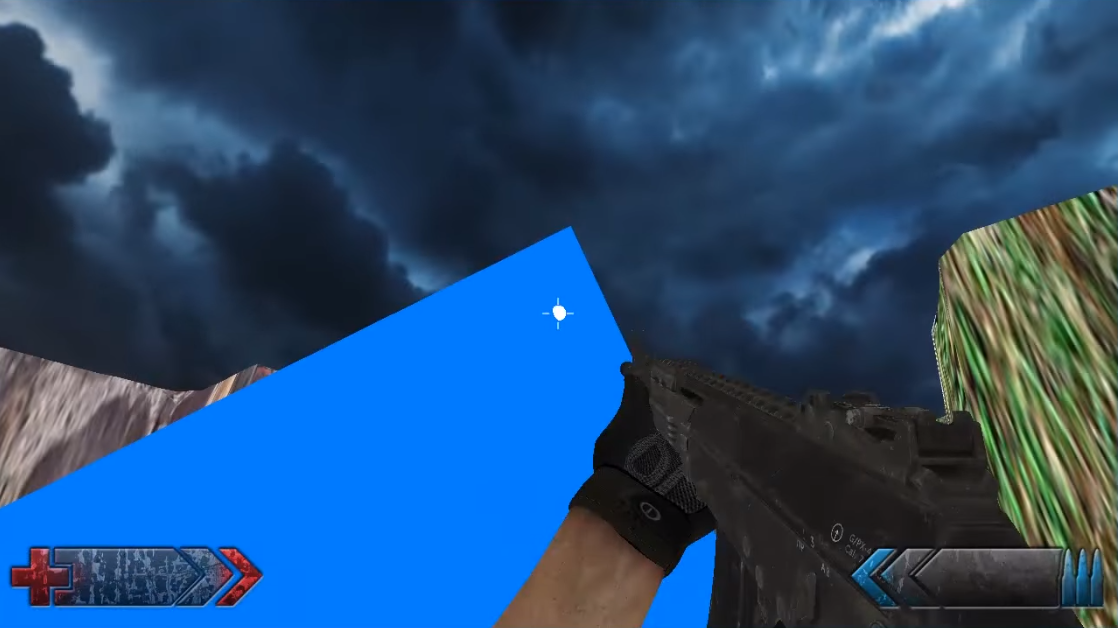
\includegraphics[scale=0.46]{kepek/one_triangle.png}
\caption{Egyenes és háromszög metszéspontja vizualizációval}
\label{fig:triangle}
\end{figure}

A számításhoz a függvény először megvizsgálja, hogy azt a síkot, amelyen a háromszög van, metszi-e az egyenes, ha nem, nem is számol tovább. Ha metszi a síkot, akkor megnézi, pontosan hol metszi azt, melyek a metszéspont $(x, y, z)$ koordinátái. Ez után már csak azt kell vizsgálni, hogy a metszéspont benne van-e a három csúcspontjával leírt háromszögben. Ha igen, akkor visszaadja a metszéspontot.

\section{A játékos, és az ellenfelek ütközésének vizsgálata}

Ennek a működése hasonló, mint a domborzat és tereptárgyak üközésvizsgálatánál, azzal a különbséggel, hogy itt azt kell vizsgálni, hogy az ellenfelek körül lévő, a játékosok számára láthatatlan hengerrel van-e metszéspontja az adott egyenesnek. Ezt a hengert nevezzük jelen esetben \textit{hitbox}-nak. Ennek a megválasztása hatással van egyrészt az ütközésvizsgálat pontosságára, másrészt pedig a számítási időre.

\begin{figure}[h]
\centering
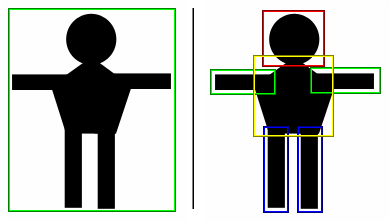
\includegraphics[scale=0.38]{kepek/hitbox.png}
\caption{Különböző részletességű hitbox-ok}
\label{fig:hitbox}
\end{figure}

A hitbox arra szolgál, hogy egy közelítő becslésünk legyen az ütközésvizsgálathoz. Amennyiben eltaláltuk egy objektum \textit{hitbox}-át, úgy meg kell vizsgálni, hogy a benne lévő modellel van-e ütközés. Amennyiben nincs, ugyanazt kell tennünk, mint ha a közelítő alakzattal sem lett volna ütközés.

% Ebben az esetben azért nem a pontos, látható geometriára számoljuk a találatokat, mert annak nagyon nagy erőforrásigénye lenne, ellenben az lenne a legpontosabb, tehát amit látunk, az jelenti a találatot. A találatszámításra használt leegyszerűsített geometria előnye, hogy sokkal kevesebb hátérszámításra van szükség. Viszont mivel nem azt találjuk el, amit látunk, előfordulhatnak kellemetlen, vagy érdekes szituációk. Előfordulhat, hogy úgy találjuk el az ellenfelet, hogy ott valójában nem látunk semmit, vagy ennek ellenkezője, hogy elvileg eltaláljuk, de az a rész nem tartozik a hitbox-hoz.

Online lövöldözős játékoknál további problémát jelenthet a hálózati kommunikációból eredő hosszú válaszidő. Ebben az esetben az ellenfél játékosok nem minden esetben azon a pozíción vannak, mint ahol látjuk őket, mivel a számunkra megjelenített helyüket a játékmotor lokálisan becsli. Amennyiben a becslés rossz volt (az ellenfél játékos más irányba mozdult el, mint ahová a kliensünk azt várta volna), az általunk leadott pontos lövést érvénytelennek kell tekinteni.

\section{Optimalizálási módszerek}

Az ütközésvizsgálatra minden képkocka kiszámítása előtt szükség van. Maga a számítás eredeti felírásában nagyon számításigényes, ezért mindenképpen szükséges, hogy ezt valahogyan optimalizáljuk. A következőkben néhány lehetséges optimalizálási módszer kerül bemutatásra.

\subsection{A játéktér szabályos felosztása}

Az optimalizálás egyik módja, hogy felosztjuk a játékteret kisebb részekre, majd ezeket olyan struktúrába rendezzük, hogy a bennük való keresés hatékonyabb legyen. Ennek egyik egyszerűbb változata, hogy egyenközű felosztást alkalmazunk. Ezt követően meg kell határoznunk, hogy melyik objektum, vagy a pályának melyik része melyik térrészben található. Egyenközű felosztásra láthatunk egy példát \aref{fig:grid}. ábrán.

A karakterek ütközésvizsgálatánál elegendő, ha mindig csak arra a térrészre vesszük figyelembe az ütközést amelyikben épp tartózkodik az objektum, de ajánlott a körülötte levő 8 részre is.

A lövedék becsapódásának $(x, y, z)$ koordinátáját is kevesebb számítással kaphatjuk meg így, mert csak azokat a térrészeket kell figyelembe venni, amelyek a játékos karakterének irányvektorával metszésben vannak. A módszer implementálása egyszerű, de mégis nagy gyorsulást tapasztalhatunk a számításokban. Hátránya viszont, hogy mindenhol egyformán osztjuk fel a teret, és lehetnek olyan részek, ahol indokolatlanul sűrű a felosztás. Ilyen például egy nagy mező, amelyen nincsenek tereptárgyak vagy egyéb objektumok. Azért, hogy a felosztott térrészekben való keresés hatékonyabb legyen, a felosztást egy fa struktúra szerint tesszük meg. A felosztásban szereplő régiók számának logaritmusával lesz majd arányos a keresés lépéseinek a száma.

\begin{figure}[h]
\centering
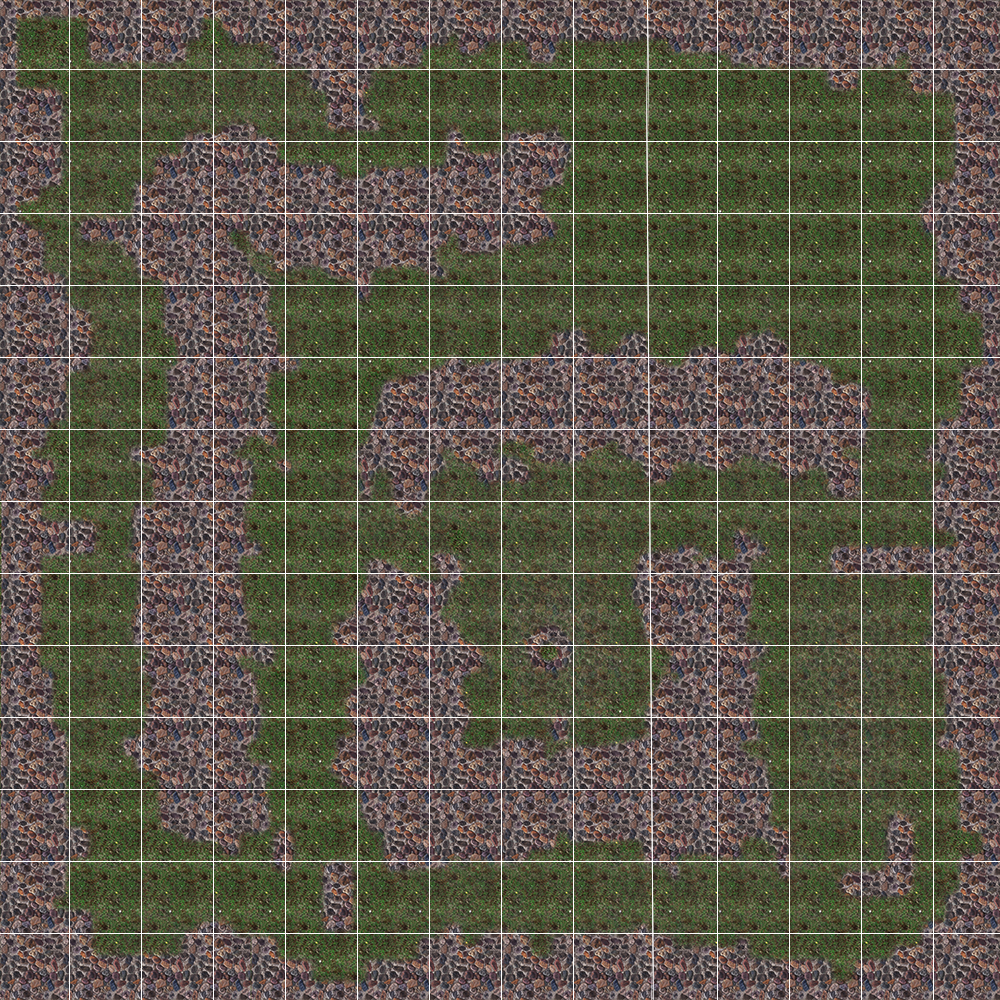
\includegraphics[scale=0.2]{kepek/grid.png}
\caption{A pálya felosztása egyenlő részekre}
\label{fig:grid}
\end{figure}

\subsection{Négyes fa és az oktális fa}

A négyes- és az oktális fa hasonló módszereket takarnak. A négyes fát síkbeli, míg az oktális fát térbeli felosztásra használják. Olyan, kivételes esetekben használható jól a négyes fa térben is, ha a játéktér nem nagy magassággal rendelkezik.

Használatánál az első feladatunk a fa gyökerének meghatározása, ami a teljes játékteret magában foglalja. Négyes fa esetén a síkot mindig 4 egyenlő részre osztjuk mindaddig, amíg a fa mélysége el nem éri a maximális, előre definiált értéket, vagy az adott cellában az objektumok száma nem lesz több, mint egy előre definiált érték. Ugyanez a megközelítés érvényesül az oktális fánál, annyi különbséggel, hogy ott 8 felé osztjuk a teret. A négyes fa felosztásainak szemléltetése \aref{fig:quadtree}. ábrán látható.

\begin{figure}[h]
\centering
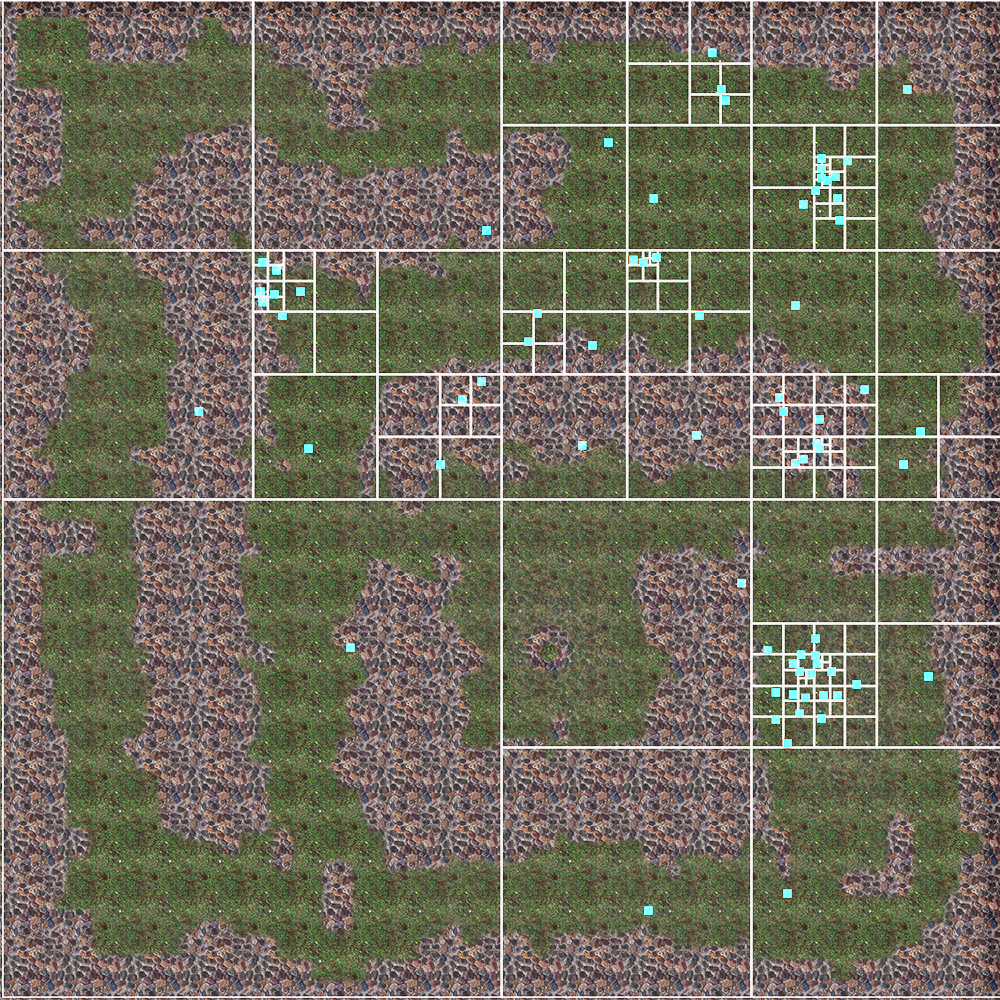
\includegraphics[scale=0.2]{kepek/quadtree.png}
\caption{A pálya felosztása a rajta lévő objektumok alapján}
\label{fig:quadtree}
\end{figure}

\subsection{A BSP fa}

A BSP (\textit{Binary Space Partitioning}) egy, a tér felezésére épülő térpartícionáló módszer. Tetszőleges dimenziójú térben alkalmazható. A BSP fa mindig két részre osztja a teret, viszont a vágósík nem a térrész mérete alapján felezi a teret, hanem a benne található objektumok száma alapján. (Páratlan elemszám esetén az egyik térrészben egyel több elem kerül.) Az osztás irányát a fa minden mélységi szintjén változtatja, egyszer vízszintes, egyszer függőleges a vágás. Az adott objektumig úgy jutunk el, hogy mindig kiválasztjuk, hogy az éppen vizsgált objektum az osztás bal, vagy jobb oldalán van. Kilépési feltételnek, szintén a négyes fához hasonlóan, megadhatjuk a fa maximális mélységét, illetve az adott cellában szereplő maximális objektumszámot. Ideális esetben a fa leveleibe egy-egy objektum kerül.

\subsection{Optimalizálási módszer kiválasztása}

A saját játékom készítése során a négyes fát alkalmaztam, hogy optimalizáljam az erőforrások felhasználását a fölösleges számítások mellőzésével, de ez a módszer felhasználható még akár egy raktárépület területének felosztására, hogy a keresést optimalizáljuk, így kevesebb időt vegyen igénybe.

Azért a négyes fa alkalmazására esett a választás, mert ezt egyszerűbb volt implementálni, és a térrész magassága eleve limitált, így a $z$ összetevőnek kisebb a jelentősége.

\subsection{Program: Négyes fa}

Megvalósítás során meg kell adnunk a gyökér csomópontot, ami a teljes, felosztani kívánt területet takarja. Egy csomópont $x$ és $y$ pozíciót, $x$ és $y$ hosszt, 4 darab gyerek node-ot (ha nincs, akkor az adott node értéke $nullptr$), illetve egy pont tömböt tartalmaz.

Meg kell adnunk az objektumok helyét, amelyeket figyelembe véve történik meg a felosztás. Ha az objektumok száma a meghatározott értéknél nagyobb, az adott node gyerek node-jai meghatározásra kerülnek. Ez az egész folyamat egy rekurzív algoritmus. Gyerek node területének meghatározásánál, mivel a területet 4 felé osztjuk, adott, hogy mindkét oldalát feleznünk kell. A for ciklusban is a terület 4 felé osztása miatt megy az i 4-ig. 

\begin{algorithm}[H]
 \KwData{node; pontok\;}
 \KwResult{A teljes terület összes része}
  \If{pontok > küszöbérték}{
   	\For{i := 0; i < 4; i++}{
   		Adott node gyerek node-jának[i] := új node;\\
   		Gyerek node területének meghatározása;\\
   		Algoritmus rekurzív hívása\;
   	}
   }
 \caption{Négyes fa területfelosztás}
\end{algorithm}

A program indítása után a felhasználó által megadott objektumok száma, a terület mérete, és az egy területben lévő maximális objektumszám megadása után elvégzi a felosztást. Eredményként ahogy \aref{fig:quad_demo}. ábrán is szerepel, láthatjuk a kialakult struktúrát.

\begin{figure}[h]
\centering
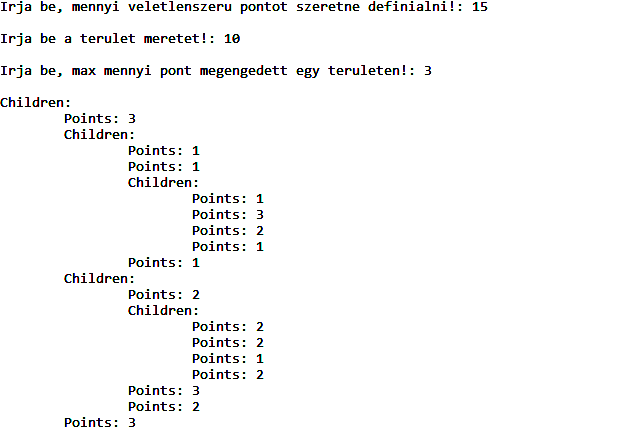
\includegraphics[scale=0.65]{kepek/quadtree_demo.png}
\caption{A négyes fa felbontással kialakult struktúra}
\label{fig:quad_demo}
\end{figure}
